\chapter{Spaces and Tensors}
\pagebreak[4]

\section{p5-exercise}

\begin{tcolorbox}

The parametric equations of a hypersurface in $V_n$ are
\begin{align*} 
\ &x^1 = a \cos(u^1)\\
\ &x^2 = a \sin(u^1)\cos(u^2)\\
\ &x^3 = a \sin(u^1)\sin(u^2)\cos(u^3)\\
\vdots\\
\ &x^{N-1} = a \sin(u^1)\sin(u^2)\sin(u^3)\dots\sin(u^{N-2})\cos(u^{N-1})\\
\ &x^{N} = a \sin(u^1)\sin(u^2)\sin(u^3)\dots\sin(u^{N-2})\sin(u^{N-1})\\
\end{align*}
where a is a constant. Find the single equation of the hyperspace in the form 1.103.

\end{tcolorbox}

We have:
\begin{align*}
\ (x^N)^2 + (x^{N-1})^2 &= a^2\prod_{i=1}^{N-2}\sin^2(u^i)(\cos^2(u^{N-1})+\sin^2(u^{N-1}))  \\
\ &= a^2\prod_{i=1}^{N-2}\sin^2(u^i)\\
\ &= a^2\prod_{i=1}^{N-3}\sin^2(u^i)\sin^2(u^{N-2})\\
\ &= a^2\prod_{i=1}^{N-3}\sin^2(u^i)(1-\cos^2(u^{N-2})\\
\ &= a^2\prod_{i=1}^{N-3}\sin^2(u^i) - a^2\prod_{i=1}^{N-3}\sin^2(u^i)\cos^2(u^{N-2})\\
\ &= a^2\prod_{i=1}^{N-3}\sin^2(u^i) - (x^{N-2})^2\\
\end{align*}
giving
$$(x^N)^2 + (x^{N-1})^2 + (x^{N-2})^2 = a^2\prod_{i=1}^{N-3}\sin^2(u^i)$$
In general, by recursion
$$\sum_{i=0}^k(x^{N-i})^2 = a^2\prod_{i=1}^{N-k-1}\sin^2(u^i)     \quad (k \leq N-2)$$
be k = N - 2 (N - k - 1 = 1) and in the left term put j = N - i (j goes from 2 to N), we get
\begin{align*}
\sum_{j=2}^N(x^{j})^2 &= a^2\prod_{i=1}^{1}\sin^2(u^i)\\
\ &= a^2(1-\cos^2(u^1))\\
\ &= a^2 - (x^1)^2\\
\end{align*}
and thus the equation of the hyperspace is given by
\begin{LARGE}
\textbf{
$$\sum_{j=1}^N(x^{j})^2 - a^2 = 0$$
}
\end{LARGE}
\begin{tcolorbox}

Determine whether the points $(\frac{1}{2}a,0,0,... 0)$, $(0,0,...,0, 2a)$ lie on the same or opposite sides of the hyperspace.
\end{tcolorbox}
For $(\frac{1}{2}a,0,0,... 0)$ we have $\sum_{j=1}^N(x^{j})^2 - a^2 = -\frac{3a^2}{4} < 0$ and for 
$(0,0,...,0, 2a)$ \\we have $\sum_{j=1}^N(x^{j})^2 - a^2 = \frac{3a^2}{4} > 0$.\\
So the points lie on opposite sides of the hyperplane.
$$\medblackdiamond$$
\pagebreak[4]

\section{p6-exercise}

\begin{tcolorbox}

Let $U_2$ and $W_2$ be subspaces of $V_N$. Show that if N = 3  they will in general intersect in a curve; if N = 4 they will in general intersect in a finite number of points; and if $N > 4$ they will not in general intersect at all.
\end{tcolorbox}

We have (see 1.102 page 5):
$\quad x^r = f^r(u^1, u^2,..., u^M) \quad (r = 1, 2, ...,N)$

Case N=3: \\

For $U_2$ we have:
$$x^r = \phi^r(u^1, u^2) \quad (r = 1, 2, 3)$$

For $W_2$ we have:
$$x^r = \psi^r(v^1, v^2) \quad (r = 1, 2, 3)$$

The intersect of the two hyperplanes is given by the N equations:

$$\phi^r(u^1, u^2) = \psi^r(v^1, v^2) \quad (r = 1, 2, 3)$$

So we have 3 equations in 4 unknown $u^1,u^2, v^1, v^2$ and can choose (fix) one e.g. $u^1$ and solve the set of equations  for $u^2, v^1, v^2$ giving 
$$x^r = \theta^r(u^1) \quad (r = 1, 2, 3)$$
This is an equation of a curve in space (1 parameter equation)\\
Case N=4: \\
Using the same reasoning as with N=3, we get 4 equations for 4 unknown $u^1,u^2, v^1, v^2$.\\
Provided that the set of equation does not degenerate, these 4 equations will determine $u^1,u^2, v^1, v^2$ without any degree of freedom. So we get  points as solutions. This solution does not to be unique, e.g. if the $\phi^r(u^1, u^2)$ are quadratic form, then the solutions 
$$(u^1,u^2, v^1, v^2)$$
$$(-u^1,u^2, v^1, v^2)$$
$$ (u^1,-u^2, v^1, v^2)$$
$$ (-u^1,-u^2, v^1, v^2)$$
are possible.\\
Case N=5: 
There are more equations than variables. If the equations are not linear dependent, no solutions will be found.
$$\medblackdiamond$$
\pagebreak[4]
\section{p8-exercise}

\begin{tcolorbox}
Show that $(a_{rst}+a_{str}+a_{srt})x^rx^sx^t = 3a_{rst}x^rx^sx^t$
\end{tcolorbox}
%\setcounter {equation} {1} %sets the counter to have the specified
$(a_{rst}+a_{str}+a_{srt})x^rx^sx^t = a_{rst}x^rx^sx^t+a_{rts}x^rx^sx^t+a_{srt}x^rx^sx^t\quad$
so by just renaming the dummy indices e.g. for the second term  $r \mapsto s\quad$, $s \mapsto t\quad$ and $t \mapsto r\quad$ we get the desired result.
$$\medblackdiamond$$
\pagebreak[4]

\section{p8-exercise}

\begin{tcolorbox}
If $\phi = a_{rs}x^rx^s$, show that
$$\pdv{\phi}{x^{r}} = (a_{rs}+a_{sr})x^s \quad\text{,}\quad\pdv{\phi}{x^{r}}{x^{s}} = a_{rs}+a_{sr}$$
Simplify these expressions in the case where $a^{rs} = a^{sr}$
\end{tcolorbox}
We have 
\begin{align} 
\pdv{\phi}{x^{t}} &= \pdv{a_{rs}}{x^{t}}x^{r}x^{s}+a_{rs}\pdv{x^{r}}{x^{t}}x^{s}+a_{rs}x^{r}\pdv{x^{s}}{x^{t}}\\
&= \pdv{a_{rs}}{x^{t}}x^{r}x^{s}+a_{rs}\delta_t^rx^{s}+a_{rs}x^{r}\delta^s_t\\
&= \pdv{a_{rs}}{x^{t}}x^{r}x^{s}+a_{ts}x^{s}+a_{rt}x^{r}\\
&= \pdv{a_{rs}}{x^{t}}x^{r}x^{s}+a_{ts}x^{s}+a_{st}x^{s}\quad\text{(rename dummy variable in third term)}\\
&= \pdv{a_{rs}}{x^{t}}x^{r}x^{s}+(a_{ts}+a_{st})x^{s}
\end{align}
Replace $x^t$ by $x^r$, we get
\begin{align}
\pdv{\phi}{x^{r}}  =\pdv{a_{rs}}{x^{r}}x^{r}x^{s}+(a_{rs}+a_{sr})x^{s}
\end{align}
So the asked expression is only true if $a_{rs}$ is not a function of the $x^{s}$.
Assuming that $a_{rs}$ is not a function of the $x^{s}$, take the partial derivative of (6) with respect to $x^{t}$, we get
\begin{align} 
\pdv{\phi}{x^{r}}{x^{t}} &= (a_{rs}+a_{sr})\pdv{x^{s}}{x^{t}}\\
&=(a_{rs}+a_{sr})\delta^{s}_{t}\\
&=(a_{rt}+a_{tr})
\end{align}
Replace $x^t$ by $x^s$, and we get the proposed expression.
$$\medblackdiamond$$
\pagebreak[4]

\section{p8-clarification on expression 1.210}

\begin{tcolorbox}
$$\pdv{x^{,q}}{x^{p}}{x^{s}}+\pdv{x^{r}}{x^{,m}}{x^{,n}}\pdv{x^{,m}}{x^{p}}\pdv{x^{,n}}{x^{s}}\pdv{x^{,q}}{x^{r}} = 0 $$
\end{tcolorbox}
From 1.209:
\begin{gather} 
\pdv{x^r}{x^{,m}}{x^{,n}}\pdv{x^{,m}}{x^{p}}\pdv{x^{,n}}{x^{s}}+\pdv{x^r}{x^{,n}}\pdv{x^{,n}}{x^p}{x^{s}} = 0
\end{gather}
 multiply (1)  with $\quad\pdv{x^{,q}}{x^{r}}$
\begin{gather} 
\pdv{x^r}{x^{,m}}{x^{,n}}\pdv{x^{,m}}{x^{p}}\pdv{x^{,n}}{x^{s}}\pdv{x^{,q}}{x^{r}}+\pdv{x^r}{x^{,n}}\pdv{x^{,n}}{x^p}{x^{s}}\pdv{x^{,q}}{x^{r}} = 0\\
\Leftrightarrow\pdv{x^r}{x^{,n}}\pdv{x^{,n}}{x^p}{x^{s}}\pdv{x^{,q}}{x^{r}}+ \pdv{x^r}{x^{,m}}{x^{,n}}\pdv{x^{,m}}{x^{p}}\pdv{x^{,n}}{x^{s}}\pdv{x^{,q}}{x^{r}}= 0
\end{gather}
\begin{gather} 
\text{\centering in the first term we get\quad\quad}\quad \pdv{x^{,q}}{x^{r}}\pdv{x^r}{x^{,n}} = \pdv{x^{,q}}{x^{,n}} = \delta_n^q
\end{gather}
(3) becomes
\begin{gather} 
\pdv{x^{,n}}{x^p}{x^{s}}\delta_n^q + \pdv{x^r}{x^{,m}}{x^{,n}}\pdv{x^{,m}}{x^{p}}\pdv{x^{,n}}{x^{s}}\pdv{x^{,q}}{x^{r}}=  0\\
\Leftrightarrow\pdv{x^{,q}}{x^p}{x^{s}} + \pdv{x^r}{x^{,m}}{x^{,n}}\pdv{x^{,m}}{x^{p}}\pdv{x^{,n}}{x^{s}}\pdv{x^{,q}}{x^{r}}= 0
\end{gather} 
$$\medblackdiamond$$
\pagebreak[4]



\section{p9-exercise}

\begin{tcolorbox}
If $A_s^r$ are the elements of a determinant A, and $B_s^r$ the elements of a determinant B, show that the element of the product determinant is $A_n^rB^n_s$. Hence show that the product of the two jacobians
$$J =\Bigg|\pdv{x^{r}}{x^{,s}}\Bigg|\text{,}\quad J^{'} = \Bigg|\pdv{x^{,r}}{x^{s}}\Bigg|$$
is unity.
\end{tcolorbox}
Remark: Some nitpick about the formulation: $A_s^r$ are not the elements of a determinant A, but elements of the matrix A which gives $\det{A}$ provided that A is square (which is not explicitly mentioned.). The same remark for B and $A_n^rB^n_s$.\\
Be $A^i_k $ the elements of matrix A and $B^k_j $ the elements of matrix B and C = A.B the resulting matrix of the multiplication of A and B, then
$$C^i_j  = A^i_kB^k_j $$
are the elements of matrix C.
Now, put $A^i_k =\pdv{x^{i}}{x^{,k}} \quad$ and $B^k_j =\pdv{x^{,k}}{x^{j}} \quad$ then,
\begin{align}
C^{i}_{j}  &= A^{i}_{k}B^{k}_{j} \\
&=\pdv{x^{i}}{x^{,k}}\pdv{x^{,k}}{x^{j}}\\
&= \delta^{i}_{k}
\end{align}
So $C = JJ^{,}\quad$becomes the unity matrix. 
$$\medblackdiamond$$
\pagebreak[4]

\section{p11-exercise}

\begin{tcolorbox}
Show that a finite contravariant vector determines the ratios of the components of an infinitesimal displacement. (Consider the transformation of the equation $dx^r=\theta T^r$, where $\theta$ is an arbitrary factor which does not change under the transformation. Alternatively, show that the equations $T^{r} dx^{s}-T^{s} x^{r} = 0$ remain true when we transform the coordinates.)

\end{tcolorbox}
Be $T^{q}$ a contravariant vector.
\begin{align}
T^{,q}=T^{r} \pdv{x^{,q}}{x^r}\quad\text{(by definition)}
\end{align}
Be  $\theta$ a small infinitesimal factor invariant for a coordinate transformation,  define \\
\begin{align}
\ dx^{r} = \theta T^{r} \\
\end{align}
then
\begin{align}
\dv{x^r}{x^s} = \frac{\theta T^r}{\theta T^s}\\
\Leftrightarrow T^s dx^r - T^r dx^s = 0
\end{align}
Alternatively, multiply (5) with $\partial_{x^r}{x^{,q}}$, then
\begin{align}
\pdv{x^{,q}}{x^r} dx^r T^s   -  \pdv{x^{,q}}{x^r}dx^s T^r &= 0\\
\Leftrightarrow \pdv{x^{,q}}{x^r} dx^r T^s   -  dx^s T^{,q} &= 0 \quad \text{(use (1) in the second term)}\\
\Leftrightarrow dx^{,q} T^s   -  dx^s T^{,q} &= 0 \\
\end{align}
Multiply (8) with $\partial_{x^s}{x^{,p}}$, then
\begin{align}
\ &dx^{,q} T^s \partial_{x^s}{x^{,p}}  -  dx^s T^{,q}\partial_{x^s}{x^{,p}} = 0 \\
\Leftrightarrow \quad &T^{,p} dx^q   -   T^{,q} dx^{,p} = 0 \quad \text{(use (1) in the first term)}
\end{align}
and thus 
$$\dv{x^{,q}}{x^{,p}} = \frac{T^{,q}}{T^{,p}}$$

$$\medblackdiamond$$
\pagebreak[4]


\section{p12-exercise}

\begin{tcolorbox}
Write down the equation of transformation, analogous to 1.305, of a contravariant tensor of the third order. Solve the equation so as to express the unprimed components in terms of the primed components.

\end{tcolorbox}
Be 
\begin{align}
T^{,uvw}=T^{rst} \pdv{x^{,u}}{x^r}\pdv{x^{,v}}{x^s}\pdv{x^{,w}}{x^t}\quad\text{(by definition)}
\end{align}
a contravariant vector.\\
Multiply (1) by $\pdv{x^{n}}{x^{,u}}$
\begin{align}
\ T^{,uvw}\pdv{x^{n}}{x^{,u}}&= T^{rst} \pdv{x^{,u}}{x^r}\pdv{x^{n}}{x^{,u}}\pdv{x^{,v}}{x^s}\pdv{x^{,w}}{x^t}\\
\Leftrightarrow  T^{,uvw}\pdv{x^{n}}{x^{,u}}&= T^{rst} \delta^{n}_{r}\pdv{x^{,v}}{x^s}\pdv{x^{,w}}{x^t}\\
\Leftrightarrow  T^{,uvw}\pdv{x^{n}}{x^{,u}}&= T^{nst} \pdv{x^{,v}}{x^s}\pdv{x^{,w}}{x^t}
\end{align}
Multiply (4) by $\pdv{x^{m}}{x^{,v}}$
\begin{align}
\ T^{,uvw}\pdv{x^{n}}{x^{,u}}\pdv{x^{m}}{x^{,v}} &= T^{nst} \pdv{x^{,v}}{x^s}\pdv{x^{m}}{x^{,v}}\pdv{x^{,w}}{x^t}\\
\Leftrightarrow  \ T^{,uvw}\pdv{x^{n}}{x^{,u}}\pdv{x^{m}}{x^{,v}} &= T^{nst} \delta_{s}^{m}\pdv{x^{,w}}{x^t}\\
\Leftrightarrow  \ T^{,uvw}\pdv{x^{n}}{x^{,u}}\pdv{x^{m}}{x^{,v}} &= T^{nmt} \pdv{x^{,w}}{x^t}
\end{align}
Multiply (7) by $\pdv{x^{p}}{x^{,w}}$
\begin{align}
\ T^{,uvw}\pdv{x^{n}}{x^{,u}}\pdv{x^{m}}{x^{,v}}\pdv{x^{p}}{x^{,w}} &= T^{nmt} \pdv{x^{,w}}{x^t}\pdv{x^{p}}{x^{,w}}\\
\Leftrightarrow \ T^{,uvw}\pdv{x^{n}}{x^{,u}}\pdv{x^{m}}{x^{,v}}\pdv{x^{p}}{x^{,w}} &= T^{nmt} \delta^{p}_{t}\\
\Leftrightarrow  \ T^{,uvw}\pdv{x^{n}}{x^{,u}}\pdv{x^{m}}{x^{,v}}\pdv{x^{p}}{x^{,w}} &= T^{nmp} 
\end{align}
Giving
$$T^{nmp} =  T^{,uvw}\pdv{x^{n}}{x^{,u}}\pdv{x^{m}}{x^{,v}}\pdv{x^{p}}{x^{,w}} $$

$$\medblackdiamond$$
\pagebreak[4]

\section{p14-exercise}

\begin{tcolorbox}
For a transformation from on set of rectangular Cartesian coordinates to another in Euclidean 3-space, show that the law of transformation of a contravariant vector is precisely the same as that of a covariant vector. Can this statements be extended to cover tensor of higher orders?
\end{tcolorbox}
We have to prove that, given that, $$T^{,i}= T^{j} \pdv{x^{,i}}{x^j} \quad T^{,}_{i}= T_{j} \pdv{x^{j}}{x^{,i}}$$ that also
\begin{align}
\ T^{,i}= T^{j} \pdv{x^{j}}{x^{,i}} \quad T^{,}_{i}&= T_{j}\pdv{x^{,i}}{x^j} \\
\Leftrightarrow \pdv{x^{j}}{x^{,i}} &= \pdv{x^{,i}}{x^j} 
\end{align}
Be
\begin{align}
\hat{e^{,i}} = g^i_k\hat{e^{k}}\quad\text{and } \hat{e^{i}} = h^i_k\hat{e^{,k}}
\end{align}
the transformation rules from one set of (rectangular Cartesian) basis vectors to another set of  (rectangular Cartesian) basis vectors.
Then,
\begin{align}
\langle \hat{e^{,i}},\hat{e^{,j}} \rangle = \langle g^i_k\hat{e^{k}},g^j_k\hat{e^{k}} \rangle &\text{ and } \langle \hat{e^{i}},\hat{e^{j}} \rangle = \langle h^i_k\hat{e^{,k}},h^j_k\hat{e^{,k}} \rangle\\
\Leftrightarrow \delta^p_j = g^p_k g^j_k &\text{ and } \delta^p_j = h^p_k h^j_k \\
\end{align}
Be $\vec{v}$ a random vector in the Euclidean space,
\begin{align}
\vec{v} = x^j\hat{e^{j}} = x^{,j}\hat{e^{,j}}
\end{align}
then
\begin{align}
\text{(3) } \Rightarrow x^j\hat{e^{j}} = x^{j}h^j_k\hat{e^{,k}}&\text{ and }x^{,j}\hat{e^{,j}} = x^{,j}g^j_k\hat{e^{k}}\\
\Rightarrow x^{,j} = x^{m}h^m_j  &\text{ and }x^m = x^{,j}g^j_m\\
\Rightarrow x^{,j} = x^{,i}g^i_m h^m_j&\text{ and } x^m = x^{k}h^k_j g^j_m \\
\Rightarrow \delta^p_j =g^p_k h^k_j &\text{ and } \delta^p_j =g^k_j h^p_k\\
\text{(5) } \Rightarrow g^p_k g^j_k=g^p_k h^k_j &\text{ and } h^p_k h^j_k=g^k_j h^p_k\\
 \Rightarrow g^j_k =  h^k_j &\text{ and }h^j_k =  g^k_j
\end{align}
From (9)
\begin{align}
\ x^{j} = x^{,m} g^m_j &\text{ and } x^{,k} = x^{n} h^n_k\\
\Rightarrow \pdv{x^{,k}}{x^j} = \pdv{x^{n}}{x^j} h^n_k  &\text{ and } \pdv{x^{j}}{x^{,k}} = \pdv{x^{,m}}{x^{,k}}g^m_j\\
\Leftrightarrow \pdv{x^{,k}}{x^j} = \delta^n_j h^n_k  &\text{ and } \pdv{x^{j}}{x^{,k}} = \delta^m_k g^m_j\\
\Leftrightarrow \pdv{x^{,k}}{x^j} = h^j_k  &\text{ and } \pdv{x^{j}}{x^{,k}} = g^k_j\\
\text{(13) }\Rightarrow \pdv{x^{,k}}{x^j} &= \pdv{x^{j}}{x^{,k}}
\end{align}
So (13) matches (2), proving the assertion.\\\\
Can this statements be extended to cover tensor of higher orders?
Consider
$$T^{,i,j,\dots ,n}= T^{r,s,\dots w} \pdv{x^{,i}}{x^{r}}\pdv{x^{,j}}{x^{s}}\dots \pdv{x^{,n}}{x^{w}} \text{ and } T^{r,s,\dots w}= T^{,i,j,\dots ,n} \pdv{x^{r}}{x^{,i}}\pdv{x^{s}}{x^{,j}}\dots \pdv{x^{w}}{x^{,n}}$$
Using the same reasoning as in (1) to (2) we need
$$\pdv{x^{,i}}{x^{r}}\pdv{x^{,j}}{x^{s}}\dots \pdv{x^{,n}}{x^{w}} =\pdv{x^{r}}{x^{,i}}\pdv{x^{s}}{x^{,j}}\dots \pdv{x^{w}}{x^{,n}}$$
As the conclusion (18) is independent of the order of the tensor, it is obvious that the above equality yields. Hence, the answer is YES.

$$\medblackdiamond$$
\pagebreak[4]

\section{p16-exercise}

\begin{tcolorbox}
In a space of 4 dimensions, the tensor $A_{rst}$ is skew-symmetric in the last pair of suffixes. Show that only 24 of the 64 components may be chosen arbitrarily. If the further condition
$A_{rst} + A_{str}+A_{trs} =0$
is imposed, show that that only 20 components may be chosen arbitrarily.

\end{tcolorbox}
We have, as A is skew-symmetric in the last pair of suffixes
$$A_{rst} = -A_{rts}  \Rightarrow s=t \text{: } A_{rst} = 0 $$
So, for each r (4 possible choices as N = 4) we have 4x4/2 - 4 = 6 degrees of freedom. [we have the term 4x4/2  as the tensor is (skew-)symmetric, e.g. once we choose element $a_{12}$, then $a_{21}$ is also known. The term -4 takes into account the diagonal element which are 0 and thus cannot be chosen.]\\
So, we have 4x6 = 24 degrees of freedom.\\
What about the supplementary constraint $A_{rst} + A_{str}+A_{trs} =0 $       :\\
Consider the two possible excluding cases:\\

i) $r=s\neq t \text{ (}\Leftrightarrow r=t\neq s \text{)}$\\
This case gives - without the additional constraint (1) -  4x(4x3/2-4) = 8 degrees of freedom.
Does the constraint (1) reduces this degree of freedom?\\
We have, 
\begin{align}
\ A_{rst} + A_{str}+A_{trs} =0\\
\Rightarrow \underbrace{A_{rrt} + A_{rtr}}_\text{= 0 (non-diagonal terms)} + \underbrace{A_{trr}}_\text{= 0 (diagonal terms)} =0
\end{align}
So, no additional constraints are added by (1) to the restriction i) and the DOF remains 8.\\

ii) $t \neq r\neq s\neq t$\\
This case means that we have to choose a set of 3 elements out of 4 elements without repetition. This a \textit{variation} of 3 elements out of 4.
$$V^n_{k} = \frac{n!}{(n-k)!} \text{ giving } V^4_{3} = \frac{4!}{(4-3)!} = 24 $$
The constraint (1) gives us 24 equations but as  $A_{rst} = -A_{rts}$ only 12 equations have to be considered. So, with the  additional constraints the DOF becomes 24-12 = 12.\\
As i) and ii) are independent and excluding events we can add the DOF of both events and we get 8+12 = 20 DOF.

$$\medblackdiamond$$
\pagebreak[4]

\section{p16-exercise}

\begin{tcolorbox}
If $A^{rs}$ is skew-symmetric and $B_{rs}$ is symmetric, prove that $A^{rs}B_{rs} = 0$. Hence show that the quadratic form $a_{ij}x^ix^j$ is unchanged if $a_{ij}$ is replaced by its symmetric part.
\end{tcolorbox}
We can split the summation $A^{rs}B_{rs}$ in three subsummations:
\begin{align}
\ A^{rs}B_{rs}  = &A^{rs}B_{rs} \vert_{r=s} \\
\ + &A^{rs}B_{rs}\vert_{r>s} \\
\ + &A^{rs}B_{rs}\vert_{r<s}
\end{align}
We have:\\
(1) = 0 as $A^{kk} = 0$ (skew-symmetric)\\
(2)+(3) = $A^{rs}B_{rs}\vert_{r>s} \ + A^{rs}B_{rs}\vert_{r<s}$\\
As $A^{rs} = -A^{sr}$ and $B^{rs} = B^{sr}$ we can write (2)+(3) as :
$$A^{rs}B_{rs}\vert_{r>s} \ + (-A^{sr})B_{sr}\vert_{r>s} = 0$$
So, $A^{rs}B_{rs} = 0$\\\\
Consider the quadratic form $\phi = a_{ij}x^ix^j$\\
Be $A_{ij} = (a_{ij})$ and $B_{ij} = (x^ix^j)$, then it is obvious that $B_{ij}$ is symmetric and that $C_{ij} = -A_{ij}$ is the form where $-a_{ij}$ is replaced by its symmetric part (skew-symmetric).
Hence $\phi = a_{ij}x^ix^j =a_{ij}b^{ij}= 0$ and so is $\phi = c_{ij}b^{ij}= 0$ 

$$\medblackdiamond$$
\pagebreak[4]

\section{p18-exercise}

\begin{tcolorbox}
What are the values (in a space of N dimensions) of the folllowing contractions formed from the Kronecker delta?
$$\delta^{m}_{m},  \delta^{m}_{n} \delta^{n}_{m},  \delta^{m}_{n} \delta^{n}_{r} \delta^{r}_{m}$$
\end{tcolorbox}
We can split the summation $A^{rs}B_{rs}$ in three subsummations:
\begin{align}
\delta^{m}_{m} = N\\
\delta^{m}_{n} \delta^{n}_{m} = \delta^{m}_{m} = N\\
\delta^{m}_{n} \delta^{n}_{r} \delta^{r}_{m} = \delta^{m}_{n} \delta^{n}_{m} = \delta^{m}_{m} = N
\end{align}
$$\medblackdiamond$$
\pagebreak[4]

\section{p19-exercise}
\begin{tcolorbox}
If $X^{r}$, $Y^{r}$ are arbitrary contravariant vectors and $a_{rs}X^{r}Y^{s}$ is an invariant, then $a_{rs}$ are the components of a covariant tensor of the second order. 
\end{tcolorbox}
We have to prove that
\begin{align}
\ a^{,}_{rs} = a_{ij}\pdv{x^{i}}{x^{,r}}\pdv{x^{j}}{x^{,s}} \text{ or } a^{}_{ij} = a^{,}_{rs}\pdv{x^{,r}}{x^{i}}\pdv{x^{,s}}{x^{j}}
\end{align}
$a_{rs}X^{r}Y^{s}$ is an invariant, means
\begin{align}
\ a^{,}_{rs}X^{,r}Y^{,s} = a_{rs}X^{r}Y^{s}
\end{align}
As $X^{r}$, $Y^{r}$ are arbitrary contravariant vectors, we have
\begin{align}
\ X^{,r} = X^{i}\pdv{x^{,r}}{x^{i}} \text{   and  } Y^{,s} = Y^{j}\pdv{x^{,s}}{x^{j}}
\end{align}
(3) in (2) gives
\begin{align}
\ a^{,}_{rs}X^{i}\pdv{x^{,r}}{x^{i}}Y^{j}\pdv{x^{,s}}{x^{j}} = a_{rs}X^{r}Y^{s}\\
\Leftrightarrow a^{,}_{rs}\pdv{x^{,r}}{x^{i}}\pdv{x^{,s}}{x^{j}}X^{i}Y^{j} = a_{ij}X^{i}Y^{j}\\
\Leftrightarrow (a^{,}_{rs}\pdv{x^{,r}}{x^{i}}\pdv{x^{,s}}{x^{j}} - a_{ij})X^{i}Y^{j} = 0
\end{align}
As $X^{r}$, $Y^{r}$ are arbitrary contravariant vectors, we conclude that 
\begin{align}
\ a^{,}_{rs}\pdv{x^{,r}}{x^{i}}\pdv{x^{,s}}{x^{j}} - a_{ij} = 0\\
\Leftrightarrow a_{ij} =  a^{,}_{rs}\pdv{x^{,r}}{x^{i}}\pdv{x^{,s}} {x^{j}}
\end{align}
(8) = (1): OK
$$\medblackdiamond$$
\pagebreak[4]

\section{p19-exercise}
\begin{tcolorbox}
If $X_{rs}$ is an arbitrary covariant tensor of the second order, and $A^{mn}_{r }X_{mn}$ is a covariant vector, then $A^{mn}_{r }$ has the mixed tensor character indicated by the positions of its suffixes 
\end{tcolorbox}
We have to prove that
\begin{align}
\ A^{,vw}_{r} = A^{mn}_k\pdv{x^{k}}{x^{,r}}\pdv{x^{,v}}{x^{m}}\pdv{x^{,w}}{x^{n}} 
\end{align}
We have
\begin{align}
\ P_{r} =A^{mn}_{r }X_{mn}
\end{align}
is a covariant vector
\begin{align}
\Rightarrow P^{,}_{r} =A^{mn}_{k }X_{mn}\pdv{x^{k}}{x^{,r}}
\end{align}
but $X_{mn}$ is a covariant tensor
\begin{align}
\Rightarrow X_{mn} = X^{,}_{ps}\pdv{x^{,p}}{x^{m}}\pdv{x^{,s}}{x^{n}}
\end{align}
So (4) in (3) gives
\begin{align}
\ P^{,}_{r} =A^{mn}_{k }X^{,}_{ps}\pdv{x^{,p}}{x^{m}}\pdv{x^{,s}}{x^{n}}\pdv{x^{k}}{x^{,r}}\\
\Leftrightarrow P^{,}_{r} = \underbrace{A^{mn}_{k }\pdv{x^{,p}}{x^{m}}\pdv{x^{,s}}{x^{n}}\pdv{x^{k}}{x^{,r}}}_\text{(*)}X^{,}_{ps}
\end{align}
Putting (*) as $ A^{,ps}_{r }= A^{mn}_{k }\pdv{x^{,p}}{x^{m}}\pdv{x^{,s}}{x^{n}}\pdv{x^{k}}{x^{,r}}$ we see that (6) has the form (2) and that $A^{,ps}_{r }$ obeys the rule of a mixed tensor (1).
$$\medblackdiamond$$
\pagebreak[4]

\section{p21-exercise}
\begin{tcolorbox}
If $A_{rs}$ is a skew-symmetric covariant tensor, prove that $B_{rst}$ defined as 
$$B_{rst} = \partial_{r}{A_{st}} + \partial_{s}{A_{tr}} +\partial_{t}{A_{rs}} $$ is a covariant tensor, and that it is skew-symmetric in all pairs of suffixes.
\end{tcolorbox}

We have $A_{rs}$ is a covariant tensor
\begin{align}
\ A_{ij} &= A_{\alpha\beta}\pdv{x^{\alpha}}{x^{i}}\pdv{x^{\beta}}{x^{j}}\\
\Rightarrow B_{rst} &= \partial_{r}{(A_{\alpha\beta}\pdv{x^{\alpha}}{x^{s}}\pdv{x^{\beta}}{x^{t}})} + \partial_{s}{(A_{\alpha\beta}\pdv{x^{\alpha}}{x^{t}}\pdv{x^{\beta}}{x^{r}})} +\partial_{t}{(A_{\alpha\beta}\pdv{x^{\alpha}}{x^{r}}\pdv{x^{\beta}}{x^{s}})}
\end{align}
Note that
\begin{align}
\partial_{k}{(A_{\alpha\beta}\pdv{x^{\alpha}}{x^{s}}\pdv{x^{\beta}}{x^{t}})} = 
\partial_{k}{(A_{\alpha\beta})}\pdv{x^{\alpha}}{x^{s}}\pdv{x^{\beta}}{x^{t}}+
\ A_{\alpha\beta}\partial_{k}{(\pdv{x^{\alpha}}{x^{s}})}\pdv{x^{\beta}}{x^{t}}+
\ A_{\alpha\beta}\pdv{x^{\alpha}}{x^{s}} \partial_{k}{(\pdv{x^{\beta}}{x^{t}})}\\
\end{align}
so, 
\begin{align}
\begin{array}{r c l}
\ B_{rst} = \partial_{r}{A_{\alpha\beta}}\pdv{x^{\alpha}}{x^{s}}\pdv{x^{\beta}}{x^{t}}+ \underbrace{A_{\alpha\beta}\partial_{r}{\pdv{x^{\alpha}}{x^{s}}}\pdv{x^{\beta}}{x^{t}}}_\text{*} +\underbrace{A_{\alpha\beta}\pdv{x^{\alpha}}{x^{s}}\partial_{r}{\pdv{x^{\beta}}{x^{t}}}}_\text{**}\\ +
\partial_{s}{A_{\alpha\beta}}\pdv{x^{\alpha}}{x^{t}}\pdv{x^{\beta}}{x^{r}}+\underbrace{A_{\alpha\beta}\partial_{s}{\pdv{x^{\alpha}}{x^{t}}}\pdv{x^{\beta}}{x^{r}}}_\text{***}+\underbrace{A_{\alpha\beta}\pdv{x^{\alpha}}{x^{t}}\partial_{s}{\pdv{x^{\beta}}{x^{r}}}}_\text{*}\\+
\partial_{t}{A_{\alpha\beta}}\pdv{x^{\alpha}}{x^{r}}\pdv{x^{\beta}}{x^{s}}+A_{\alpha\beta}\underbrace{\partial_{t}{\pdv{x^{\alpha}}{x^{r}}}\pdv{x^{\beta}}{x^{s}}}_\text{**}+\underbrace{A_{\alpha\beta}\pdv{x^{\alpha}}{x^{r}}\partial_{t}{\pdv{x^{\beta}}{x^{s}}}}_\text{***}
\end{array}
\end{align}
In (5) consider the two terms with (*) 
\begin{align}
\ T &= A_{\alpha\beta}\partial_{r}{\pdv{x^{\alpha}}{x^{s}}}\pdv{x^{\beta}}{x^{t}}+ A_{\alpha\beta}\pdv{x^{\alpha}}{x^{t}}\partial_{s}{\pdv{x^{\beta}}{x^{r}}}\\
& = A_{\alpha\beta}\pdv{x^{\alpha}}{x^{s}}{x^{r}}\pdv{x^{\beta}}{x^{t}}+ A_{\alpha\beta}\pdv{x^{\alpha}}{x^{t}}\pdv{x^{\beta}}{x^{r}}{x^{s}}\\
& = A_{\alpha\beta}\pdv{x^{\alpha}}{x^{s}}{x^{r}}\pdv{x^{\beta}}{x^{t}}+ A_{\beta\alpha}\pdv{x^{\beta}}{x^{t}}\pdv{x^{\alpha}}{x^{r}}{x^{s}} \text{ (by renaming dummy variables)}
\end{align}
As $A_{ij} = - A_{ji}$ (skew-symmetric tensor), we get $T=0$. The same yields for the (**) and (***) terms. So, $B_{rst}$ reduces to
\begin{align}
\ B_{rst} = \partial_{r}{A_{\alpha\beta}}\pdv{x^{\alpha}}{x^{s}}\pdv{x^{\beta}}{x^{t}}+ 
\partial_{s}{A_{\alpha\beta}}\pdv{x^{\alpha}}{x^{t}}\pdv{x^{\beta}}{x^{r}}+
\partial_{t}{A_{\alpha\beta}}\pdv{x^{\alpha}}{x^{r}}\pdv{x^{\beta}}{x^{s}}\\
\Leftrightarrow \ B_{rst} = \pdv{A_{\alpha\beta}}{x^{\gamma}}\pdv{x^{\gamma}}{x^{r}}\pdv{x^{\alpha}}{x^{s}}\pdv{x^{\beta}}{x^{t}}+ 
\pdv{A_{\alpha\beta}}{x^{\gamma}}\pdv{x^{\gamma}}{x^{s}}\pdv{x^{\alpha}}{x^{t}}\pdv{x^{\beta}}{x^{r}}+
\pdv{A_{\alpha\beta}}{x^{\gamma}}\pdv{x^{\gamma}}{x^{t}}\pdv{x^{\alpha}}{x^{r}}\pdv{x^{\beta}}{x^{s}}
\end{align}
By adequate renaming of the dummy variable in the 3 terms:
$$  \left[ {\begin{array}{c}
    1^{st} term \\
    2^{nd} term  \\
    3^{rd} term  
  \end{array} } \right]
\longrightarrow
  \left[ {\begin{array}{ccc}
    \gamma \to \alpha & \alpha \to \beta & \beta \to \gamma \\
    \beta \to \alpha & \gamma \to \beta & \alpha \to \gamma \\
    \alpha \to \alpha & \beta \to \beta & \gamma \to \gamma 
  \end{array} } \right]
$$
we get
\begin{align}
\ B_{rst} = (\pdv{A_{\beta\gamma}}{x^{\alpha}}+\pdv{A_{\gamma\alpha}}{x^{\beta}}+\pdv{A_{\alpha\beta}}{x^{\gamma}})\pdv{x^{\alpha}}{x^{r}}\pdv{x^{\beta}}{x^{s}}\pdv{x^{\gamma}}{x^{t}}\\
\Leftrightarrow  B_{rst} = (\underbrace{\partial_{\alpha}{A_{\beta\gamma}}+\partial_{\beta}{A_{\gamma\alpha}}+\partial_{\gamma}{A_{\alpha\beta}}}_\text{(****)})\pdv{x^{\alpha}}{x^{r}}\pdv{x^{\beta}}{x^{s}}\pdv{x^{\gamma}}{x^{t}}
\end{align}
The expression (****) has exactly the required form $B_{rst} = \partial_{r}{A_{st}} + \partial_{s}{A_{tr}} +\partial_{t}{A_{rs}} $ and is transformed (12) according the rules of a covariant tensor.\\
Let's prove now that it is skew-symmetric in all pairs of suffixes.
We have to consider the following permutations
$$  \left[ {\begin{array}{c}
    rst \\
    rts\\
    srt  \\
    str\\  
    trs \\
    tsr
  \end{array} } \right]$$
  
E.g. $srt$
\begin{align}
\ B_{rts} &= \partial_{r}{A_{ts}}+\partial_{t}{A_{sr}}+\partial_{s}{A_{rt}}\\
&= -\partial_{r}{A_{st}}-\partial_{t}{A_{rs}}-\partial_{s}{A_{tr}}\\
&= - B_{rst}
\end{align}
The same calculations can be done for the other permutations.
$$\medblackdiamond$$
\pagebreak[4]

\section{p23-exercise 1.}
\begin{tcolorbox}
In a $V_{4}$ there are two 2-spaces with equations
$$x^r = f^r(u^1,u^2)\text{, }x^r = g^r(u^3,u^4) $$
Prove that if these 2-spaces have a curve of intersection, then the determinal equation
$$\left|\pdv{x^r}{u^s}\right| = 0$$
is satisfied along the curve.
\end{tcolorbox}
Having a curve means that one of the parameters $u^i$ can be freely chosen while the other 3 are determined by the chosen parameter.\\
We have,
\begin{align}
\left|\pdv{x^r}{u^s}\right| = \left| {\begin{array}{cccc}
    \pdv{x^1}{u^1} & \pdv{x^1}{u^2} & \pdv{x^1}{u^3} & \pdv{x^1}{u^4}\\
    \vdots & \vdots & \vdots & \vdots\\
    \pdv{x^4}{u^1} & \pdv{x^4}{u^2} & \pdv{x^4}{u^3} & \pdv{x^4}{u^4}\\
  \end{array} } \right|
\end{align}
Suppose we choose $u^4$ as parameter.
This means $u^i = \phi^i(u^4)$ for i=1,2,3 and thus we can write
\begin{align}
\pdv{x^i}{u^4} &= \pdv{x^i}{u^j}\dv{\phi^j}{u^4}+ \pdv{x^i}{u^4}\quad\text{ with j=1,2,3} \quad\text{  i = 1,2,3,4}\\
&\Rightarrow \pdv{x^i}{u^j}\dv{\phi^j}{u^4} = 0
\end{align}
This means that in (1) the three first columns a not linearly independent and thus have   $\left|\pdv{x^r}{u^s}\right| = 0$

$$\medblackdiamond$$
\pagebreak[4]

\section{p23-exercise 2.}
\begin{tcolorbox}
In Euclidean space of three dimensions, write down the equations of transformation between rectangular Cartesian coordinates x, y, z and spherical polar coordinates $r$,$\theta$,$\phi$.\\
Find the Jacobian of the transformation. Where is it zero or infinite?
\end{tcolorbox}

\begin{figure}[h]
\centering
\begin{minipage}[t]{.5\textwidth}
%\centering
\vspace{0pt}
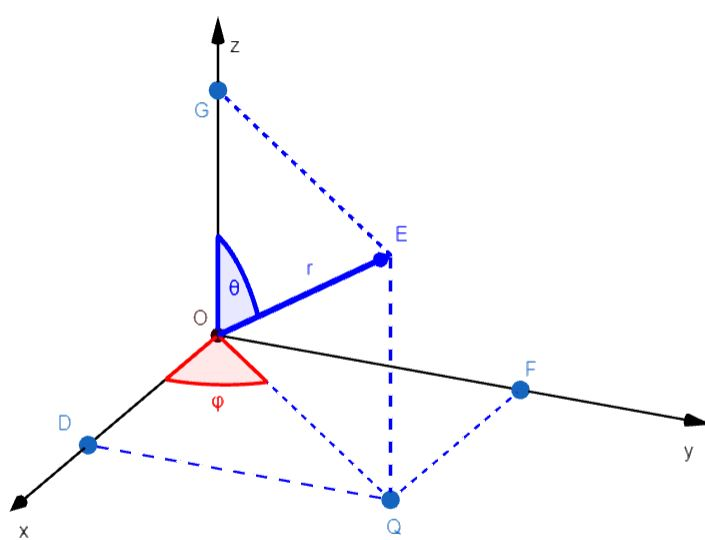
\includegraphics[scale=.5]{spherical.jpg}
\end{minipage}\hfill
\begin{minipage}[t]{0.4\textwidth}
%\centering
\vspace{50pt}
We use the latitude $\psi$ instead of the co-latitude $\phi$.\\\\
$\left\{ \begin{array}{c}
    x= r\cos (\psi )\cos (\theta) \\
     y= r\cos (\psi )\sin (\theta) \\
      z= r\sin(\psi )
  \end{array} \right\}$
\end{minipage}
\end{figure}
Partial differentiating of (x,y,z) with respect to (r,$\psi$,$\theta$) gives the Jacobian
\begin{align}
\ J=
\left| {\begin{array}{ccc}
    \cos (\psi )\cos (\theta) & -r\sin (\psi )\cos (\theta) & -r\cos (\psi )\sin (\theta)\\
    \cos (\psi )\sin (\theta) & -r\sin (\psi )\sin (\theta) & r\cos (\psi )\cos (\theta)\\
    \sin (\psi ) & r\cos (\psi )& 0\\
  \end{array} } \right|
\end{align}



\begin{eqnarray}
\ J &=& \cos(\psi)\cos(\theta)(-r^{2})\cos^{2}(\psi)\cos(\theta))\\ &+& r\sin(\psi) \cos(\theta)(-r\cos(\psi)\cos(\theta)\sin(\psi)) \\&-& r\cos(\psi)\sin(\theta)(r\cos^{2}(\psi)\sin(\theta)+r\sin^{2}(\psi)\sin(\theta))\\
&=& -r^{2}\cos^{3}(\psi)\cos^{2}(\theta)
-r^{2}\sin^{2}(\psi)\cos^{2}(\theta)\cos(\psi)-r^{2}\cos(\psi)\sin^{2}(\theta)
\end{eqnarray}



Noting that the $2^{nd}$ term in (5) can be written as $-r^{2}\cos^{2}(\theta)\cos(\psi)+r^{2}\cos^{2}(\theta)\cos^{3}(\psi)$, we get
\begin{align}
\ J &=  -r^{2}(\cos^{3}(\psi)\cos^{2}(\theta)+\cos^{2}(\theta)\cos(\psi)-\cos^{3}(\psi)\cos^{2}(\theta)+\cos(\psi)\sin^{2}(\theta))\\
\ &= -r^{2}\cos(\psi)
\end{align}
J=0: for $r=0$ or $\psi = \frac{\pi}{2}|_{r \epsilon (-\infty, +\infty)}$ and $J\rightarrow \pm\infty$ or $\mp\infty$ for $r\rightarrow \pm\infty|_{\psi\neq 0}$. But what about the case $r\rightarrow \pm\infty|_{\psi\rightarrow 0}$? This case is not determined as long as no path is chosen in the $(r,\psi)$ configuration space.
$$\medblackdiamond$$
\pagebreak[4]

\section{p23-exercise 3.}
\begin{tcolorbox}
If $X, Y,Z$ are the components of a contravariant vector for rectangular Cartesian coordinates in Euclidean 3-space, find it's components for spherical polar coordinates.
\end{tcolorbox}

Be $x^{\alpha}$ the components of a contravariant vector in spherical polar coordinates and $x^{i}$ it's components in rectangular Cartesian coordinates. As we have  
\begin{align}
 \begin{array}{c}
    \ x^{\rho} = \sqrt{x^{j}x^{j}}\\
    \ x^{\theta} = \atan{\frac{x^{2}}{x^{1}}}\\
    \ x^{\phi} = \asin{\frac{x^{3}}{\sqrt{{x^{j}x^{j}}}}}\\
  \end{array} \quad \text{ and } \quad A^{\alpha} = A^{i}\pdv{x^{\alpha}}{x^{i}}
  \end{align}
\begin{align}
\Rightarrow \left[A^{\alpha} \right]=  \left[A^{i}\pdv{x^{\alpha}}{x^{i}}\right] = \left[ {\begin{array}{ccc}
    \ \frac{x^1} { \sqrt{x^{j}x^{j}}} & \frac{x^2} { \sqrt{x^{j}x^{j}}} & \frac{x^3} { \sqrt{x^{j}x^{j}}}\\\\
    -\frac{x^2} { (x^1)^2+(x^2)^2} & \frac{x^1} { (x^1)^2+(x^2)^2}  & 0 \\\\
    -\frac{x^3x^1} { (x^{j}x^{j})\sqrt{(x^1)^2+(x^2)^2}} & -\frac{x^3x^2} { (x^{j}x^{j})\sqrt{(x^1)^2+(x^2)^2}}  & \frac{\sqrt{(x^1)^2+(x^2)^2}} { (x^{j}x^{j})} \\
  \end{array} } \right]\left[ {\begin{array}{c}
    \ A^{1}\\\\
    \ A^{2}\\\\
    \ A^{3}\\\\
  \end{array} } \right]
\end{align}
$$\medblackdiamond$$
\pagebreak[4]

\section{p23-exercise 4.}
\begin{tcolorbox}
In a space of three dimensions, how many different expressions are represented by the product $A^{m}_{np} B^{pq}_{rs}C^{s}_{tu}$? How many terms occur in each such expression, when written out explicitly?
\end{tcolorbox}

As we have $V_{3}$ and considering that in $A^{m}_{np} B^{pq}_{rs}C^{s}_{tu}$ the six indices m, n, q, r, t, u are not dummy indices, we get $3^{6}$ different expressions (first choose m: you have three choices, then n: also three choices giving 3x3 possibilities, etc for q, r, t, u).\\
For the second question, as in $A^{m}_{np} B^{pq}_{rs}$ there is only summation on over index (p) we get three terms for this part. As the summation with $A^{m}_{np} B^{pq}_{rs}$ and $C^{s}_{tu}$ occurs only on one index also (s) we get 3x3 terms in the expression.

$$\medblackdiamond$$
\pagebreak[4]

\section{p23-exercise 5.}
\begin{tcolorbox}
If A  is an invariant in $V_{n}$, are the second derivatives $\pdv{A}{x^{r}}{x^{s}}$ the components of a tensor?
\end{tcolorbox}

As A is invariant (note: different alphabets in the indices indicates different coordinate systems):
\begin{align}
\ A(x^{\rho}) = A(x^{i})\\
\Rightarrow \pdv{A(x^{\rho})}{x^{i}} = \pdv{A(x^{j})}{x^{i}}
\end{align}
To simplify the notation, we put $A(x^{\rho}) = A^{,}$ and $A(x^{j}) = A^{,}$ then (2) can be written as
\begin{align}
\pdv{A^{,}}{x^{\rho}}\pdv{x^{\rho}}{x^{i}} = \pdv{A}{x^{i}}
 \end{align}
 Conclusion: $\pdv{A}{x^{i}}$ is a covariant tensor. \\\\Consider now $\pdv{A}{x^{i}} = \pdv{A^{,}}{x^{\rho}}\pdv{x^{\rho}}{x^{i}}$. Then,
\begin{align}
\pdv{A}{x^{i}}{x^{j}} &= \pdv{A^{,}}{x^{\rho}}{x^{j}}\pdv{x^{\rho}}{x^{i}}+ \pdv{A^{,}}{x^{\rho}}\pdv{x^{\rho}}{x^{i}}{x^{j}}\\
\Leftrightarrow \pdv{A}{x^{i}}{x^{j}} &= \pdv{A^{,}}{x^{\rho}}{x^{\gamma}}\pdv{x^{\gamma}}{x^{j}}\pdv{x^{\rho}}{x^{i}}+ \pdv{A^{,}}{x^{\rho}}\pdv{x^{\rho}}{x^{i}}{x^{j}}
\end{align}
The first term on the right side, behaves as covariant tensor but the presence of the second term makes that generally, $\pdv{A}{x^{i}}{x^{j}}$ has not a tensor character. This is only when $\pdv{A^{,}}{x^{\rho}}\pdv{x^{\rho}}{x^{i}}{x^{j}}=0$, which means that $x^{\rho}, x^{i}$ are a linear map of each other.
$$\medblackdiamond$$
\pagebreak[4]

\section{p23-exercise 6.}
\begin{tcolorbox}
Suppose that in $V_2$ the components of a contravariant tensor field $T^{mn}$ in a coordinate system $x^r$ are 
$$T^{11}=1 \quad T^{12}=0$$
$$T^{21}=1 \quad T^{22}=0$$
Find the components $T^{,mn}$ in a coordinate system $x^{,r}$, where
$$x^{,1} =(x^{1})^2\quad x^{,2} = (x^{2})^2$$
Write down the values of these components in particular at the point $x^1 = 1, x^2 0 =$.
\end{tcolorbox}
As we have a contravariant tensor field :
\begin{align}
\ T^{,mn} =  T^{ij}\pdv{x^{,m}}{x^{i}}\pdv{x^{,n}}{x^{j}}\\
 \begin{array}{ccc}
   \quad \quad \quad \quad  x^{,1} =(x^{1})^2  \Rightarrow & \pdv{x^{,1}}{x^{1}} = 2x^{1} & \pdv{x^{,1}}{x^{2}} = 0\\
\quad \quad \quad \quad x^{,2} =(x^{2})^2  \Rightarrow & \pdv{x^{,2}}{x^{1}} = 0 & \pdv{x^{,2}}{x^{2}} = 2x^{2}\\
  \end{array}\\
  \end{align}
  \begin{align}
  &\Rightarrow T^{,11} = 4(x^{1})^2 + 4(x^{2})^2 \\
  &\Rightarrow T^{,12} = T^{,21}=0 \\
  &\Rightarrow T^{,22} = 4(x^{1})^2 + 4(x^{2})^2
  \end{align}\\\\
  The components in  at the point $x^1 = 1, x^2 = 0$ are
  $$T^{,}(1,0) = \left[{\begin{array}{cc} 4 & 0 \\
    0 & 4 \\ 
    \end{array} } \right]$$
    
    $$\medblackdiamond$$
\pagebreak[4]

\section{p24-exercise 7.}
\begin{tcolorbox}
Given that if $T_{mnrs}$ is a covariant tensor, and 
$$ T_{mnrs}+T_{mnsr} = 0$$ in a coordinate system $x^{p}$, establish directly that $$ T^{,}_{mnrs}+T^{,}_{mnsr} = 0$$ in any other coordinate system $x{,q}$.
\end{tcolorbox}
Note: in the following, different alphabets in the indices indicates different coordinate systems.
As we $T_{mnrs}$ is a covariant tensor :
\begin{align}
\ T_{\alpha\beta\gamma\delta} &=  T_{mnrs}\pdv{x^{m}}{x^{\alpha}}\pdv{x^{n}}{x^{\beta}}\pdv{x^{r}}{x^{\gamma}}\pdv{x^{s}}{x^{\delta}}\\
\Rightarrow T_{\alpha\beta\gamma\delta}+T_{\alpha\beta\delta\gamma} &= T_{mnrs}\pdv{x^{m}}{x^{\alpha}}\pdv{x^{n}}{x^{\beta}}\pdv{x^{r}}{x^{\gamma}}\pdv{x^{s}}{x^{\delta}}+ T_{mnrs}\pdv{x^{m}}{x^{\alpha}}\pdv{x^{n}}{x^{\beta}}\pdv{x^{r}}{x^{\delta}}\pdv{x^{s}}{x^{\gamma}}
\end{align}
Now, swap the dummy indices r and s in the second term on the right and as $T_{mnrs} = - T_{mnsr}$:
\begin{align}
\ T_{\alpha\beta\gamma\delta}+T_{\alpha\beta\delta\gamma} &= T_{mnrs}\pdv{x^{m}}{x^{\alpha}}\pdv{x^{n}}{x^{\beta}}\pdv{x^{r}}{x^{\gamma}}\pdv{x^{s}}{x^{\delta}}+ T_{mnsr}\pdv{x^{m}}{x^{\alpha}}\pdv{x^{n}}{x^{\beta}}\pdv{x^{s}}{x^{\delta}}\pdv{x^{r}}{x^{\gamma}}\\
&= (T_{mnrs}+ T_{mnsr})\pdv{x^{m}}{x^{\alpha}}\pdv{x^{n}}{x^{\beta}}\pdv{x^{s}}{x^{\delta}}\pdv{x^{r}}{x^{\gamma}}\\&=0
\end{align}
$$\medblackdiamond$$
\pagebreak[4]

\section{p24-exercise 8.}
\begin{tcolorbox}
Prove that if $A_{r}$ is a covariant vector, then $\pdv{A_{r}}{x^{s}} - \pdv{A_{s}}{x^{r}}$ is a skew-symmetric covariant tensor of the second order (use the notation of 1.7).
\end{tcolorbox}
Be $B_{rs} = \pdv{A_{r}}{x^{s}} - \pdv{A_{s}}{x^{r}}$.\\
i) $B_{rs}$ is skew-symmetric:
It is obvious that:$$-B_{rs} = -\pdv{A_{r}}{x^{s}} + \pdv{A_{s}}{x^{r}} = \pdv{A_{s}}{x^{r}}-\pdv{A_{r}}{x^{s}}\equiv B_{sr}$$
ii)  $B_{rs}$ is covariant:\\
\textit{Note: in the following, different alphabets in the indices indicates different coordinate systems.}\\
Let 
\begin{align}
\ C_{\alpha\beta} = (\partial_sA_r - \partial_rA_s)X^r_{\alpha}X^s_{\beta}. 
\end{align}
We know that $A_i= A_{\gamma}X^{\gamma}_i$  as $A_i$ is covariant. Hence,
\begin{align}
\partial_jA_i &= \partial_j A_{\gamma} X^{\gamma}_i + A_{\gamma}\partial_jX^{\gamma}_i\\
\ &= \partial_{\alpha} A_{\gamma} X^{\alpha}_j X^{\gamma}_i + A_{\gamma}\partial_jX^{\gamma}_i
\end{align}
Using (3), we compute the first term in (1)
\begin{align}
\partial_sA_rX^r_{\alpha}X^s_{\beta}&=  \partial_{\rho} A_{\gamma} X^{\rho}_s X^{\gamma}_rX^r_{\alpha}X^s_{\beta}+A_{\gamma}\partial_sX^{\gamma}_rX^r_{\alpha}X^s_{\beta}\\
\ &=  \partial_{\rho} A_{\gamma} X^{\rho}_{\beta} X^{\gamma}_{\alpha}+A_{\gamma}\partial_sX^{\gamma}_rX^r_{\alpha}X^s_{\beta}\\
\ &=  \partial_{\rho} A_{\gamma} \delta^{\rho}_{\beta} \delta^{\gamma}_{\alpha}+A_{\gamma}\partial_sX^{\gamma}_rX^r_{\alpha}X^s_{\beta}\\
\ &=  \partial_{\beta} A_{\alpha} +A_{\gamma}\partial_sX^{\gamma}_rX^r_{\alpha}X^s_{\beta}
\end{align}
In the same way, we get for the second term in (1)
\begin{align}
\partial_rA_sX^s_{\alpha}X^r_{\beta} &=  \partial_{\alpha} A_{\beta} + A_{\gamma}\partial_rX^{\gamma}_sX^r_{\alpha}X^s_{\beta}
\end{align}\\
And thus,
\begin{align}
\ C_{\alpha\beta} =(\partial_sA_r - \partial_rA_s)X^r_{\alpha}X^s_{\beta} &=\partial_{\beta} A_{\alpha} +A_{\gamma}\partial_sX^{\gamma}_rX^r_{\alpha}X^s_{\beta} - \partial_{\alpha} A_{\beta} - A_{\gamma}\partial_rX^{\gamma}_sX^r_{\alpha}X^s_{\beta}\\
\ \Rightarrow \partial_{\beta} A_{\alpha}  - \partial_{\alpha} A_{\beta} &=  (\partial_sA_r - \partial_rA_s)X^r_{\alpha}X^s_{\beta}
\end{align}
So, i) and (10) proves that $\pdv{A_{r}}{x^{s}} - \pdv{A_{s}}{x^{r}}$ is skew-symmetric tensor of the second order.
$$\medblackdiamond$$
\pagebreak[4]

\section{p24-exercise 9.}
\begin{tcolorbox}
Let $x^r, \overline{x}^r, y^r,\overline{y}^r $ be four systems of coordinates. Examine the tensor character of $\pdv{x^r}{y^s}$ with respect to the following transformations:\\
i) A transformation $x^r = f^r(\overline{x}^1,\dots,\overline{x}^N)$, with $y^r$ unchanged;\\
ii) A transformation $y^r = g^r(\overline{y}^1,\dots,\overline{y}^N)$, with $x^r$ unchanged;
\end{tcolorbox}
\textit{Note: in the following, different alphabets in the indices indicates different coordinate systems.}\\\\
%Be $A(r,s) = \pdv{x^r}{y^s}$.\\
i) Let's compute the expression $A(\alpha, \beta) = \pdv{x^r}{y^s}\pdv{x^{\alpha}}{x^r}\pdv{x^s}{x^{\beta }}$. Obviously, the right side is an expression of a (possible) mixed tensor of the second order ($\pdv{x^r}{y^s}$) under transformation from the (r) coordinate system to the ($\alpha$) coordinate system. Then, 
\begin{align}
\ A(\alpha, \beta) &= \pdv{x^r}{y^s}\pdv{x^{\alpha}}{x^r}\pdv{x^s}{x^{\beta }}\\
&= \pdv{x^{\alpha}}{y^s}\pdv{x^s}{x^{\beta }}\\
&= \pdv{x^{\alpha}}{y^{\rho}}\pdv{y^{\rho }}{y^s}\pdv{x^s}{x^{\beta }}
\end{align}
If we consider the $\overline{y}^r$ coordinate system as the $y^{\rho }$ coordinate system and as $\overline{y}^r = y^r$ then $\pdv{y^{\rho }}{y^s} = \delta^{\rho}_s$ and we get from (3)
\begin{align}
\ A(\alpha, \beta) &= \pdv{x^{\alpha}}{y^{\rho}}\pdv{y^{\rho }}{y^s}\pdv{x^s}{x^{\beta }}\\
\ &= \pdv{x^{\alpha}}{y^{\rho}}\delta^{\rho}_{s}\pdv{x^s}{x^{\beta }}\\
\ &= \pdv{x^{\alpha}}{y^{\rho}}\pdv{x^{\rho}}{x^{\beta }}\\
\ &= \pdv{x^{\alpha}}{y^{\rho}}\delta^{\rho}_{\beta }\\
\ &= \pdv{x^{\alpha}}{y^{\beta}}\\
\text{(1) and (8)   } \Rightarrow \pdv{x^{\alpha}}{y^{\beta}} &= \pdv{x^r}{y^s}\pdv{x^{\alpha}}{x^r}\pdv{x^s}{x^{\beta }}
\end{align}
So $A(r,s) = \pdv{x^r}{y^s}$ is a mixed tensor of type $A_s^r$\\\\
ii) Let's compute the expression $A(\alpha, \beta) = \pdv{x^r}{y^s}\pdv{y^{\alpha}}{y^r}\pdv{y^s}{y^{\beta }}$. Obviously, the right side is an expression of a (possible) mixed tensor of the second order ($\pdv{x^r}{y^s}$) under transformation from the (r) coordinate system to the ($\alpha$) coordinate system. Then, 
\begin{align}
\ A(\alpha, \beta) &= \pdv{x^r}{y^s}\pdv{y^{\alpha}}{y^r}\pdv{y^s}{y^{\beta }}\\
&= \pdv{x^r}{y^{\rho}}\pdv{y^{\rho}}{y^s}\pdv{y^{\alpha}}{y^r}\pdv{y^s}{y^{\beta }}\\
&= \pdv{x^r}{y^{\rho}}\pdv{y^{\rho}}{y^{\beta}}\pdv{y^{\alpha}}{y^r}\\
&= \pdv{x^r}{y^{\rho}}\delta^{\rho}_{\beta}\pdv{y^{\alpha}}{y^r}\\
&= \pdv{x^r}{y^{\beta}}\pdv{y^{\alpha}}{y^r}\\
&= \pdv{x^r}{x^{\sigma}}\pdv{x^{\sigma}}{y^{\beta}}\pdv{y^{\alpha}}{y^r}
\end{align}
If we consider the $\overline{x}^r$ coordinate system as the $x^{\sigma }$ coordinate system and as $\overline{x}^r = x^r$ then $\pdv{x^{\sigma }}{x^r} = \delta^{\sigma}_r$ and we get from (15)
\begin{align}
\ A(\alpha, \beta) &= \pdv{x^r}{x^{\sigma}}\pdv{x^{\sigma}}{y^{\beta}}\pdv{y^{\alpha}}{y^r}\\
\ &= \delta^r_{\sigma}\pdv{x^{\sigma}}{y^{\beta}}\pdv{y^{\alpha}}{y^r}\\
\ &= \pdv{x^{\sigma}}{y^{\beta}}\pdv{y^{\alpha}}{y^{\sigma}}\\
\ &= \pdv{x^{\sigma}}{y^{\beta}}\delta^{\alpha}_{\sigma}\\
\ &= \pdv{x^{\alpha}}{y^{\beta}}\\
\text{(10) and (19)   } \Rightarrow \pdv{x^{\alpha}}{y^{\beta}} &= \pdv{x^r}{y^s}\pdv{y^{\alpha}}{y^r}\pdv{y^s}{y^{\beta }}
\end{align}
So $A(r,s) = \pdv{x^r}{y^s}$ is a mixed tensor of type $A_s^r$
$$\medblackdiamond$$
\pagebreak[4]

\section{p23-exercise 10.}
\begin{tcolorbox}
If $x^r, y^r, z^r$ are three systems of coordinates, prove the follwoing rule for the multiplication of Jacobians.
$$\left|\pdv{x^m}{y^n}\right|\left|\pdv{y^r}{z^s}\right| = \left|\pdv{x^t}{z^u}\right|$$
\end{tcolorbox}
 As we have  
\begin{align}
\pdv{x^t}{z^u} &=\pdv{x^t}{y^k} \pdv{y^k}{z^u}\\
 \left[ { \begin{array}{ccc}
   \ \pdv{x^1}{z^1} & \dots & \pdv{x^1}{z^N}\\
   \vdots & \vdots & \vdots\\
    \pdv{x^N}{z^1} & \dots & \pdv{x^N}{z^N}\\
  \end{array}} \right] &= \left[ { \begin{array}{ccc}
   \ \pdv{x^1}{y^k}\pdv{y^k}{z^1} & \dots & \pdv{x^1}{y^k}\pdv{y^k}{z^N}\\
   \vdots & \vdots & \vdots\\
    \pdv{x^N}{y^k}\pdv{y^k}{z^1}& \dots & \pdv{x^N}{y^k}\pdv{y^k}{z^N}\\
  \end{array}} \right]\\
  &= \left[ { \begin{array}{ccc}
   \ \pdv{x^1}{y^1}& \dots & \pdv{x^1}{y^N}\\
   \vdots & \vdots & \vdots\\
    \pdv{x^N}{y^1}& \dots & \pdv{x^N}{y^k}\\
  \end{array}} \right]\left[ { \begin{array}{ccc}
   \ \pdv{y^1}{z^1} & \dots & \pdv{y^1}{z^N}\\
   \vdots & \vdots & \vdots\\
    \pdv{y^N}{z^1}& \dots & \pdv{y^N}{z^N}\\
  \end{array}} \right]\\
  \ & \Rightarrow \left|\pdv{x^m}{y^n}\right|\left|\pdv{y^r}{z^s}\right| = \left|\pdv{x^t}{z^u}\right|
  \end{align}
$$\medblackdiamond$$
\pagebreak[4]


\section{p23-exercise 11.}
\begin{tcolorbox}
Prove that with respect to transformations $$ x^{,r} = C_{rs}x^s$$ where the coefficients are constants satisfying $$C_{mr}C_{ms} = \delta^r_s$$ contravariant and covariant vectors have the same formula of transformation $$ A^{,r} = C_{rs}A^{s} \text{, } A_{,r} = C_{rs}A_{s} $$
\end{tcolorbox}
 i) $ A^{,r} = C_{rs}A^{s}$\\
 
 Be $ A^{,r} = A^{s}\pdv{x^{,r}}{x^s}$ and as $x^{,r} = C_{rs}x^{s}$  we have $\pdv{x^{,r}}{x^s} = C_{rs}$. Hence,$$ A^{,r} = C_{rs}A^{s}$$.\\\\
 i) $ A_{,r} = C_{rs}A_{s}$\\
 Be $ A_{,r} = A_{s}\pdv{x^{s}}{x^{,r}}$ and as $x^{,r} = C_{rs}x^{s}$  we have
\begin{align}
\pdv{x^{,r}}{x^{,t}} &= C_{rs}\pdv{x^{s}}{x^{,t}}\\
\Rightarrow \delta^{r}_{t} &= C_{rs}\pdv{x^{s}}{x^{,t}}
  \end{align}
  Now, multiply (2) by $C_{rq}$. We get,
  \begin{align}
 \delta^{r}_{t}C_{rq} &= C_{rq}C_{rs}\pdv{x^{s}}{x^{,t}}\\
 \ C_{tq} &= C_{rq}C_{rs}\pdv{x^{s}}{x^{,t}}\\
 \text{as }C_{mr}C_{ms} = \delta^r_s \Rightarrow \quad \quad  C_{tq} &= \delta^q_s\pdv{x^{s}}{x^{,t}}\\
 \Rightarrow   C_{tq} &= \pdv{x^{q}}{x^{,t}} \text{  or  }  C_{rs} = \pdv{x^{s}}{x^{,r}}\\
 \text{  as  } A_{,r} = A_{s}\pdv{x^{s}}{x^{,r}} \Rightarrow A_{,r} &= C_{rs}\pdv{x^{s}}{x^{,r}}
  \end{align}
$$\medblackdiamond$$
\pagebreak[4]


\section{p23-exercise 12.}
\begin{tcolorbox}
Prove that $$\pdv{ln\left|\pdv{x^m}{y^n}\right|}{x^r} =\pdv{y^m}{x^r}{x^n}\pdv{x^n}{y^m}$$.
\end{tcolorbox}
Lemma:\\
Be $A$ a square matrix $NxN$; Be $f$ a $C^1$ function $f:\mathbb{R}^{NxN} \rightarrow \mathbb{R}$. \\Define $A^{,}$ as $(A^,_{ij}) = \dv{f}{A_{ij}}$. Then,$$(ln\left|A\right|)^, = (A^{-1})^T \text{ wih }  f =\left|A\right|$$
Proof:\\
By definition of the determinant, we have
\begin{align}
\left|A\right| = A_{iK}C_{K}^i \quad \text{ (no summation on K!)}
\end{align}
with $(C_{K}^i) =  (-1)^{i+K}M^{i}_K$ being the cofactor  of element $A_{iK}$ and $M^{i}_K$ the minor (N-1)x(N-1) matrix associated with the cofactor $A_{K^i}$. Be $C = (C_{ij})$ the NxN matrix formed with all posssible cofactor elements  $C_{j}^i \text{  }(i,j = 1 \dots,N)$.\\
We have 
\begin{align}
\ A^{-1} &= \frac{C^T}{\left|A\right|}\\
\Rightarrow (A^{-1})^T &= \frac{C}{\left|A\right|} \\
\text{differentiating (1) }\Rightarrow \pdv{\left|A\right|}{A_{mn}} &= \pdv{A_{iK}}{A_{mn}}C^i_K +A_{iK} \pdv{C^i_K}{A_{mn}}\\
\text{we have for i = m } & \begin{array}{c}
    \pdv{A_{iK}}{A_{mn}} = 1\quad K=n\\
    \pdv{A_{iK}}{A_{mn}} = 0\quad K \neq n\\
  \end{array}
\end{align}
Also, $\forall K: \pdv{C^i_K}{A_{in}} = 0 $ as by definition of the cofactor matrix, $A_{ij} $ is not contained in $C_{ij} $.Hence, (4) becomes
\begin{align}
\pdv{\left|A\right|}{A_{ij}} &= C^i_j\\
\text{But,}\quad \pdv{ln\left|A\right|}{A_{ij}} &= \frac{\pdv{\left|A\right|}{A_{ij}}}{\left|A\right|}\\
\text{(6) and  (7) gives}\quad \pdv{ln\left|A\right|}{A_{ij}} &= \frac{C^i_j}{\left|A\right|}\\
\text{(3) and  (8) gives}\quad \pdv{ln\left|A\right|}{A_{ij}} &= \frac{(A^{-1}_{ij})^T \left|A\right|}{\left|A\right|} = (A^{-1}_{ij})^T \\
\Rightarrow (ln\left|A\right|)^, &= (A^{-1})^T
\end{align}\\\\
Now the main proof:\\
Let, 
\begin{align}
\ A \equiv \left[ a_{mn}\right] &= \left[ \pdv{y^m}{x^n}\right]\\
\Rightarrow \pdv{ln\left|A\right|}{x^r} &= \sum_{m,n = 1}^{N,N} \pdv{ln\left|A\right|}{a_{mn}}\pdv{a_{mn}}{x^r}\\
\text{from (10) we get }\quad \pdv{ln\left|A\right|}{a_{mn}} &= (A^{-1})^T_{mn}\\
\text{But A is a Jacobian, so } (A^{-1})_{mn} &= \pdv{x^m}{y^n}\\
\text{ and thus  }(A^{-1})^T_{mn} &=  \pdv{x^n}{y^m}\\
\text{(13) can be written as }  \pdv{ln\left|A\right|}{x^r} &=  \sum_{m,n = 1}^{N,N} \pdv{x^n}{y^m}\pdv{a_{mn}}{x^r}\\
\Rightarrow \pdv{ln\left|A\right|}{x^r} &=  \sum_{m,n = 1}^{N,N} \pdv{x^n}{y^m}\pdv{y^m}{x^r}{x^n}
\end{align}
$$\medblackdiamond$$
\pagebreak[4]
